\documentclass{article}

% if you need to pass options to natbib, use, e.g.:
%     \PassOptionsToPackage{numbers, compress}{natbib}
% before loading neurips_2021

% ready for submission
\usepackage{neurips_2021}

% to compile a preprint version, e.g., for submission to arXiv, add add the
% [preprint] option:
%     \usepackage[preprint]{neurips_2021}

% to compile a camera-ready version, add the [final] option, e.g.:
%     \usepackage[final]{neurips_2021}

% to avoid loading the natbib package, add option nonatbib:
%    \usepackage[nonatbib]{neurips_2021}

\usepackage[utf8]{inputenc} % allow utf-8 input
\usepackage[T1]{fontenc}    % use 8-bit T1 fonts
\usepackage{hyperref}       % hyperlinks
\usepackage{url}            % simple URL typesetting
\usepackage{booktabs}       % professional-quality tables
\usepackage{amsfonts}       % blackboard math symbols
\usepackage{nicefrac}       % compact symbols for 1/2, etc.
\usepackage{microtype}      % microtypography
\usepackage{xcolor}         % colors
\usepackage{graphicx}
\usepackage{amsmath}
\usepackage{float}
\graphicspath{{../img/}}
\title{Big data bowl 2022}

% The \author macro works with any number of authors. There are two commands
% used to separate the names and addresses of multiple authors: \And and \AND.
%
% Using \And between authors leaves it to LaTeX to determine where to break the
% lines. Using \AND forces a line break at that point. So, if LaTeX puts 3 of 4
% authors names on the first line, and the last on the second line, try using
% \AND instead of \And before the third author name.

\author{
	Massimo Hong\\
	Student id: 2020280082\\
	Lohan Meunier\\
	Student id: 2021280356\\
	Department of Computer Science\\
	Tsinghua University\\
 } 

\begin{document}

\maketitle

\begin{abstract}
  NFL is one of the biggest and most prestigious sport league in the United States, with the highest average attendance of any sport in the world. \\
This competition proposes 3 potential topics to study, and it is advised to examine one of them thoroughly rather than several. We chose to work on the third one which is to rank special teams’ players as it seemed very clear and feasible. We feel like the biggest challenge of this topic is to manage coming up with original ideas. If, eventually, we aren’t able to do so we would then consider changing topic for one of the other two.
Before deeply diving into the project, the subject required a lot of reading and documentation.
Because we were not familiar with American football and its rules, we studied the sport and especially special teams since it is the topic of the competition. Being an Analytics competition, it requires a very good understanding of the game, of the strategies used. We might even want to come up with new strategies depending on our results.\\
To rank and compare special teams’ players, we want to find for each of the special teams’ positions a way to grade each player (using different provided and relevant parameters). For each position, the way of grading will not be the same. And then, still by position, we will rank the players.
\end{abstract}
\section{Introduction to NFL}
The National Football League (NFL) is a professional American football league consisting of 32 teams, divided equally between the National Football Conference (NFC) and the American Football Conference (AFC). The NFL is one of the four major North American professional sports leagues, the highest professional level of American football in the world. \\
The NFL's eighteen-week regular season runs from early September to early January, with each team playing seventeen games and having one bye week. Following the conclusion of the regular season, seven teams from each conference (four division winners and three wild card teams) advance to the playoffs, a single-elimination tournament culminating in the Super Bowl, which is usually held on the first Sunday in February and is played between the champions of the NFC and AFC.
\section{Dataset}
The dataset is divided into multiple csv files:
\begin{itemize}
\item games.csv and players.csv provide very generic data on NFL games and on the players involved in special teams plays. Nothing of major interest to analyse the plays themselves, and the consequences of different parameters on the result.
\item plays.csv, it provides a lot of details on special teams plays which occurred in NFL games. It gives the context of the play (time of the game, score before the play, location of the play…), its details (play type, players involved…), and its outcome (result, penalties, yards gained…). Using this data, we could already start analysing the impact the context of the play has on its result, or the accuracy of different players.
\item racking.csv (3 files for the 3 last seasons: 2018, 2019, 2020), these ones give even more details on the different plays. They give specific data on each player involved in a play at each second (position, speed, direction of motion…). With this data we could be able to reconstitute completely the plays and the positions and choices of each player. 
\item PFF, this is probably the most important file at our disposal. It provides data on football specific metrics which are critical for a team success, especially on special teams plays. It gives us data on all the parameters that could influence the result of a play (either kickoff or punt): snap accurate or not, time between snap and kick, type of kick, duration the ball stays in the air, direction intended… This data is key if we want to quantify special teams’ strategies, compare their results. But also, to compare players and mostly kickers.
\end{itemize}
\section{Potential tasks of the competition}
\begin{itemize}
\item Create a new special teams metric.
\item Quantify special teams strategy. Special teams’ coaches are among the most creative and innovative in the league. Compare and contrast how each team game plans. Which strategies yield the best results? What are other strategies that could be adopted?
\item Rank special teams players. Each team employs a variety of players (including longsnappers, kickers, punters, and other utility special teams players). How do they stack up with respect to one another?
\end{itemize}
\section{Task 3: Player comparison by position}
Physical attributes are a big factor in American football. First of all, we started analysing the height and weight of players in the same position in order to have a better understanding of their physical qualities.\\
Here are the bar charts for height and weight of players in the 'SS' position. Note that there are some errors in the original dataset. Some players have 0 height and some of the values are incorrect, such as $height = 70$, when it should be measured in feet. 
\begin{figure}[H]
	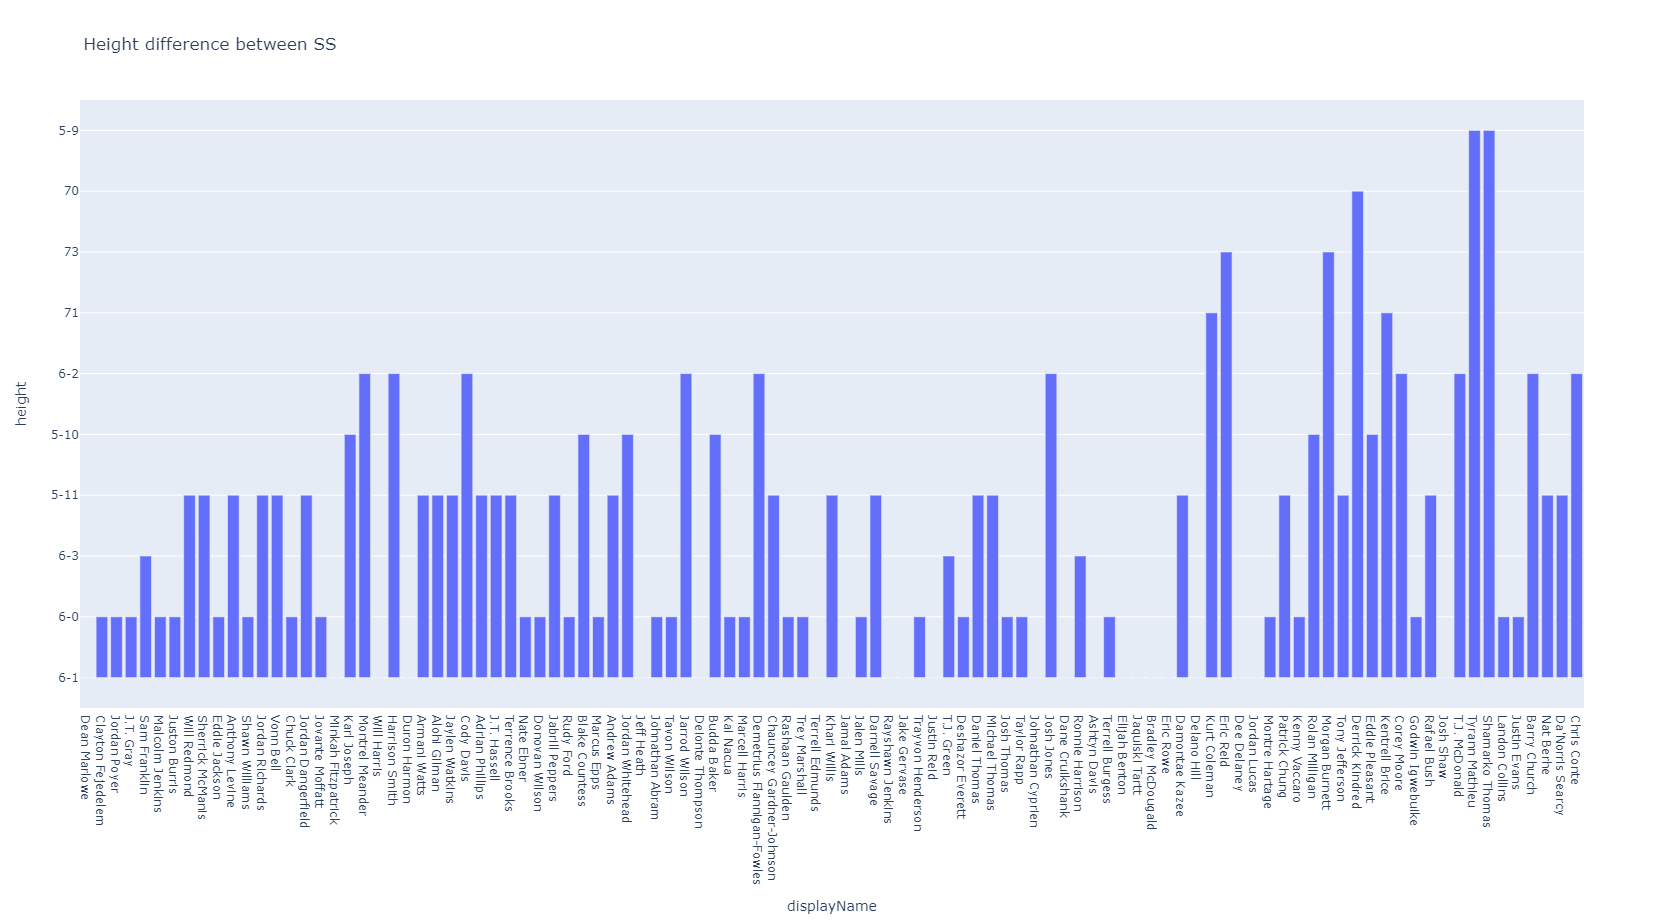
\includegraphics[width=\linewidth,height=\textheight,keepaspectratio]{height.png}
	\caption{Height of SS player(feet)}
\end{figure} 
\begin{figure}[H]
	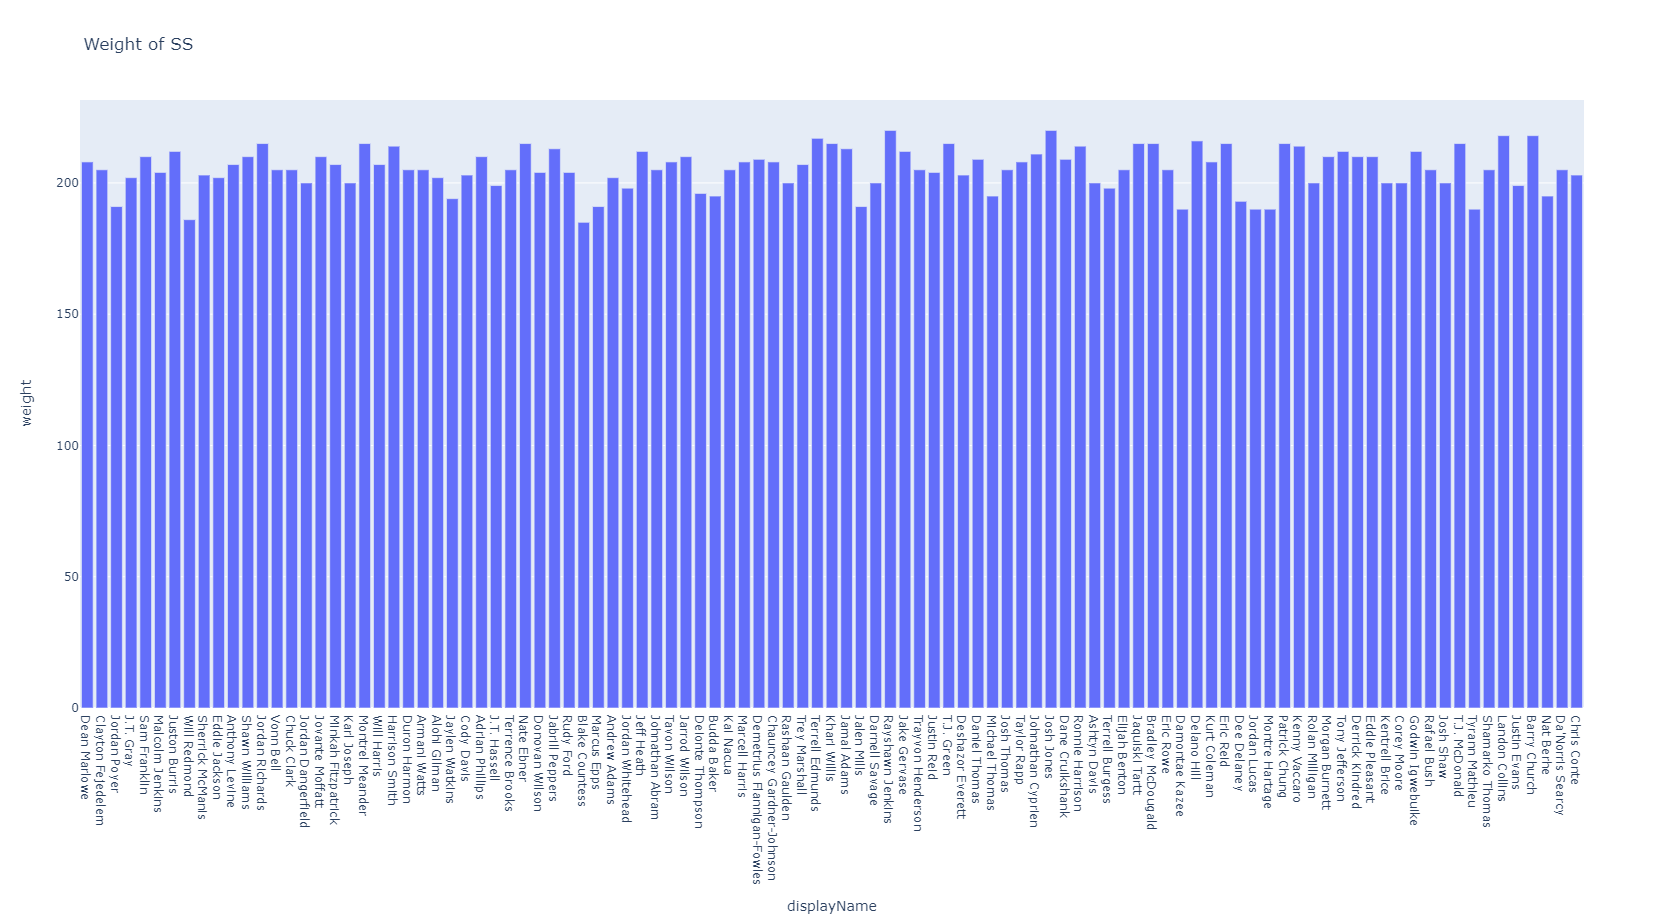
\includegraphics[width=\linewidth,height=\textheight,keepaspectratio]{weight.png}
	\caption{Weight of SS player(lbs)}
\end{figure} 
Next, we analyzed the plays a player of a certain position executed in the 2018 season.  Players and play are identified respectively by the keys nflId and playId. The $tracking_2018.csv$ contains all the details of the 2018 season.\\
In this example we have gathered all the player in the "SS" position and analized the number of unique plays they have done in the 2018 season.\\ In order to do so we have made a query in the players.csv to get the nflId of all players of said position. Next, we selected the Ids present in both players.csv and tracking 2018.csv (this way, we have found all the SS players who have played in the 2018 season) and found the number of unique plays they have executed. Below is a graphic that displays the number of unique plays each player has done. The x axis represents the nflId, while the y axis the number of plays.
\begin{figure}[H]
	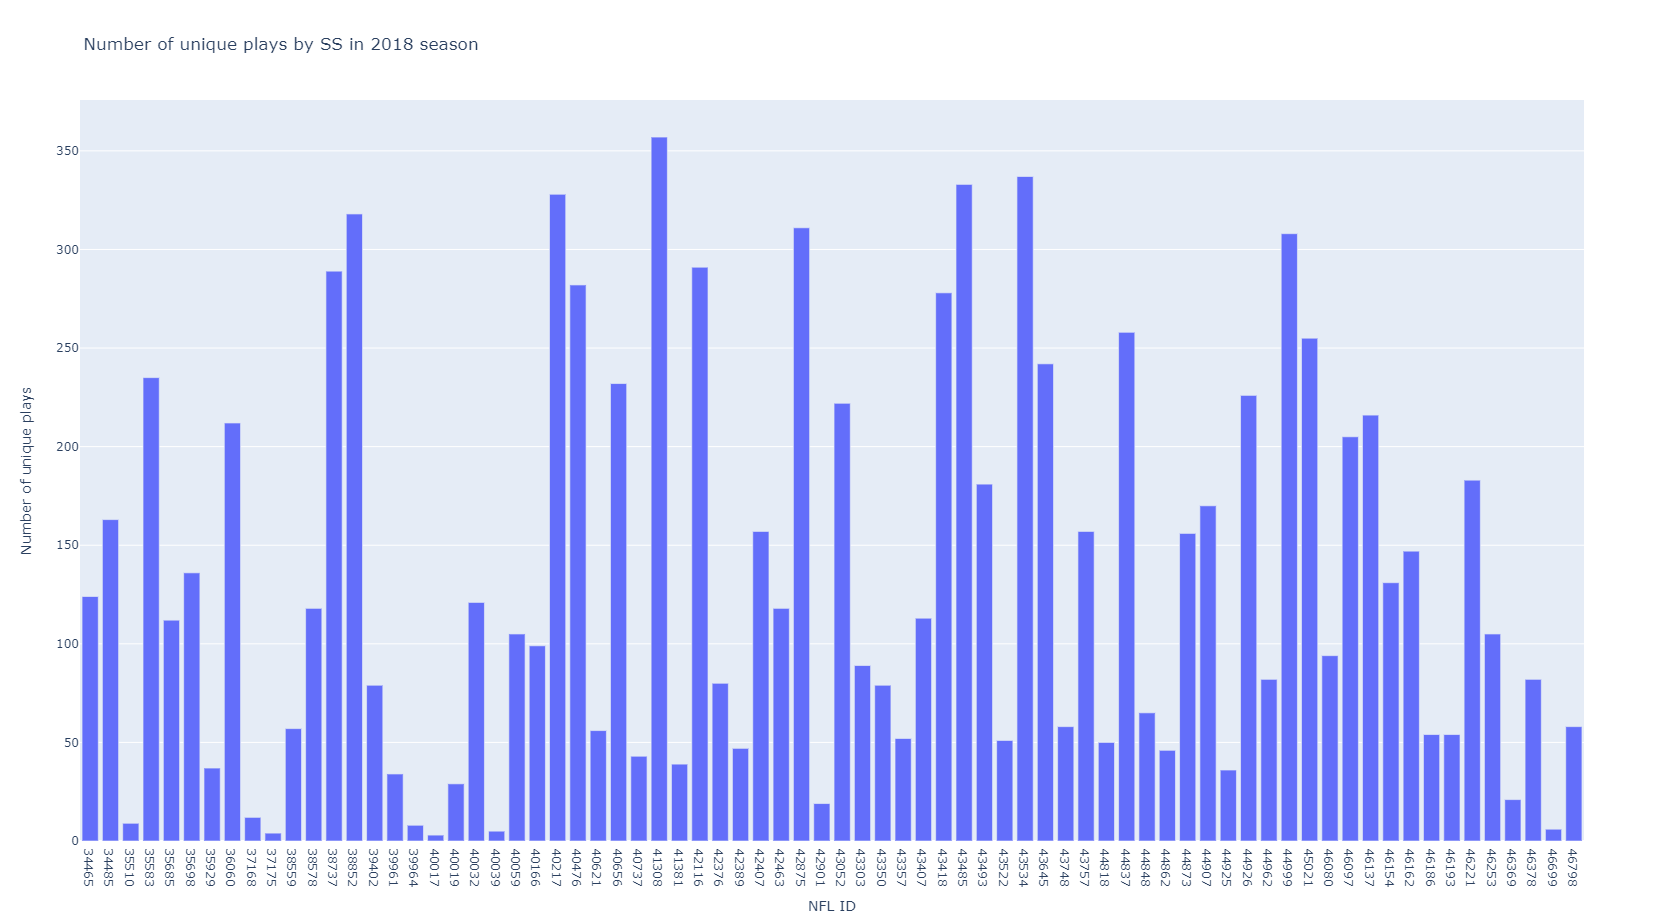
\includegraphics[width=\linewidth,height=\textheight,keepaspectratio]{SS_unique_plays_2018.png}
	\caption{Number of unique plays on SS in 2018}
\end{figure}

\section{Regression Model}
We have used a multivariate linear regression model on the followin numberical columns of the plays.csv file to predict the play result:
\begin{itemize}
	\item playId,
	\item quarter,
	\item down,
	\item yardsToGo,
	\item kickerId,
	\item penaltyYards,
	\item preSnapHomeScore,
	\item kickLength,
	\item absoluteYardlineNumber.
\end{itemize}
The NaN values present in some of the columns have been replaced by 0.
The dataset has been divided into $\frac{2}{3}$ train set and $\frac{1}{3}$ test set. After fitting the model on the train set, we performed the prediction on the test set, obtaining the following values:\\
$intercept = -5.014696885949839 $\\
$slope = [-2.43807983e-03  1.82287538e+00  6.76387035e-01  1.16248815e-01
  9.32323477e-05  1.31911354e+00  6.02097301e-02  5.91721982e-01
 -2.49419762e-03]$\\
Predicted play results $= [25. 40. 29. ... -1. -1. 43.]$
\section{Conclusion}
As of right now we are trying to anylize the ranking between players as it seems clear and feasible. We don't exclude the possibilty of changing topic in the future.
\end{document}